\documentclass[czech,bachelor]{../../shared/diploma}

\usepackage[autostyle=true,czech=quotes]{csquotes} % korektni sazba uvozovek, podpora pro balik biblatex
\usepackage[backend=biber, style=iso-numeric, alldates=iso]{biblatex} % bibliografie
\usepackage{dcolumn} % sloupce tabulky s ciselnymi hodnotami
\usepackage{subfig} % makra pro "podobrazky" a "podtabulky"
%TODO kdyžtak změn cestu kam se ti to buildi
\usepackage[outputdir=./build]{minted} % vkladani zdrojovych kodu 
\usepackage{float} % lepsi umistovani obrazku (H)

% Pozadovane vstupy pro generovani titulnich stran.
\ThesisAuthor{Miroslav Osoba}
\ThesisSupervisor{Ing. Radoslav Fasuga, Ph.D.}

\CzechThesisTitle{Tvorba uživatelského prostředí výpravné evoluční hry}
\EnglishThesisTitle{Creation of the User Environment for the Narrative Evolution Game}

\SubmissionYear{2024}

\ThesisAssignmentFileName{../specification.pdf}

\Acknowledgement{TODO Acknowledgement}

\CzechAbstract{TODO Cz Abstract}
\CzechKeywords{hybridní desková hra; uživatelské prostředí}

\EnglishAbstract{TODO En Abstract}
\EnglishKeywords{hybrid board game; user environment}

\addbibresource{resources/sauce.bib}

% Novy druh tabulkoveho sloupce, ve kterem jsou cisla zarovnana podle desetinne carky
\newcolumntype{d}[1]{D{,}{,}{#1}}

% Uprava hloubky obsahu - pozdeji smazat !
\setcounter{tocdepth}{2}


% Zacatek dokumentu
\begin{document}

% Titulni strany
\MakeTitlePages

% Seznam obrazku
\listoffigures
\clearpage

% Seznam tabulek
% \listoftables
% \clearpage

% Text zaverecne prace.
\chapter{Úvod}

Welcome to hell. This is the introduction chapter.

\chapter{Hybridní hry}
Hybridní hry kombinují jak prvky fyzické, tak digitální. Jedná se o~hry, které mají jakékoliv napojení na technologii, ať už je to elektronické bankovnictví ve hře \textit{Monopoly Super Electronic Banking} či mobilní aplikace \textit{Pokémon GO}, která uživatele pomocí map navádí k~navštívení památek a~zajímavých míst. Podobná spojení vyústí ve zcela nové herní zážitky, které si hráči mohou vyzkoušet. \cite{hybrid_board_games_design}

\section{Vývoj hybridních her}
První hybridní hry se začaly formovat již na začátku 20. století, kdy se začaly objevovat první hry s~elektronickými prvky. Tyto hry byly většinou jednoduché elektrické obvody, které hráč propojoval pro různé efekty. V~průběhu času se tyto hry stávaly složitějšími a~začaly se objevovat takové, které využívaly počítačové technologie. Hybridní hry mohou být kategorizovány do několika skupin, které se liší podle toho, jakým způsobem technologie využívají. \cite{history_of_hybrid_games}

\subsection{Stolní hry s~vlastním zařízením}
Mezi takovéto hry patří již výše zmíněné \textit{Monopoly Super Electronic Banking}, které obsahují elektronické bankovnictví, nebo známá hra \textit{Operation}, ve které se hráči nesmí dotknout kovových částí na hrací desce, jinak se rozezní siréna. 

Tato kategorie hybridních her je rozhodně nejstarší. První hrou využívající elektrického proudu, a~tudíž zařazenou do hybridních her, je hra \textit{Electra} (původním názvem \textit{Lichtra}), kterou můžeme vidět na Obrázku \ref{fig:electra}. Jedná se o~jednoduchou kvízovou hru, která vyšla už v~roce 1910 v~Německu a~byla vytvořena společností \textit{Sala Games}. Hra obsahovala jednoduchý elektrický obvod, který se uzavřel, pokud hráč odpověděl správně. Po ní následovala dlouhá éra her, jejichž elektronika také spočívala pouze v~propojení jednoho či několika málo obvodů. \cite{history_of_hybrid_games, boardgames_with_apps}

\begin{figure}[H]
    \centering
    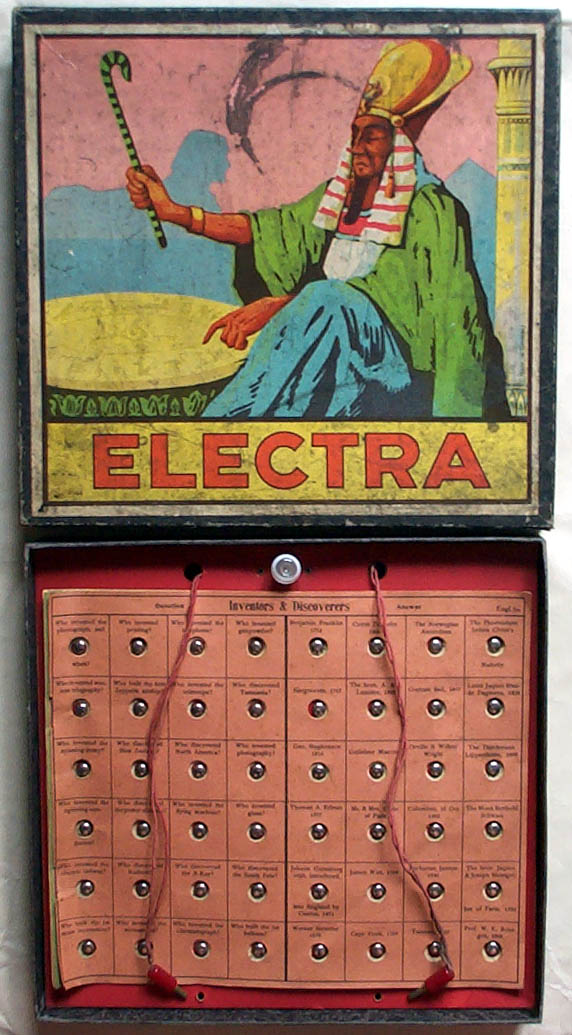
\includegraphics[width=0.3\textwidth]{resources/figures/electra.jpg}
    \caption{Hra \textit{Electra}, první hybridní hra \cite{history_of_hybrid_games}}
    \label{fig:electra}
\end{figure}

Další zmínku ve vývoji her v~této kategorii si zasloužila hra \textit{Voice of the Mummy}, která vyšla v~roce 1971. Ta měla v~herním plánu zabudovaný přehrávač, který měl simulovat hlas mumie, která při přechodu přes určitá herní pole hráčům určovala další postup. \cite{voice_of_the_mummy}

První hrou, která ve svém designu používala počítačové zařízení, byla francouzská hra \textit{Simulateur JR10}, která vyšla v~roce 1972. Jednalo se o~bitevní hru, ve které hráči ovládali různé bojové jednotky. Při střetu se do počítače vložil děrný štítek s~odpovídajícími jednotkami a~počítač podle naprogramovaných kritérií náhodně určil výsledek střetu. \cite{simulateur_jr10}

\subsection{Stolní hry s~vlastní aplikací}
V~roce 1972 vyšla herní konzole \textit{Magnavox Odyssey}, která je uznávaná jako první domácí herní konzole na světě. Zároveň s~ní vyšlo i~několik her, které kombinovaly fyzickou hrací desku s~počítačovým programem. Celé UI této konzole zahrnovalo pouze několik svítících bodů na obrazovce, proto byl ke každé hře přiložen lehce průsvitný plán s~potiskem, který se na obrazovku přichytil. Součástí většiny her byly i~fyzické komponenty, které měly hráčům sloužit k~přirozenějšímu pozvolnému přechodu ze stolních her na hry digitální. \cite{magnavox_odyssey} Jednou z~her vytvořenou pro tuto konzoli byla hra \textit{Invasion}, jejíž fyzická složka zahrnovala kostky, sadu karet, sadu tokenů a~hrací desku. Samotný program byl pak určen k~soubojům mezi hráči. Tyto komponenty můžeme vidět na Obrázku \ref{fig:invasion} \cite{invasion,invasion_gameplay}

\begin{figure}[H]
    \centering
    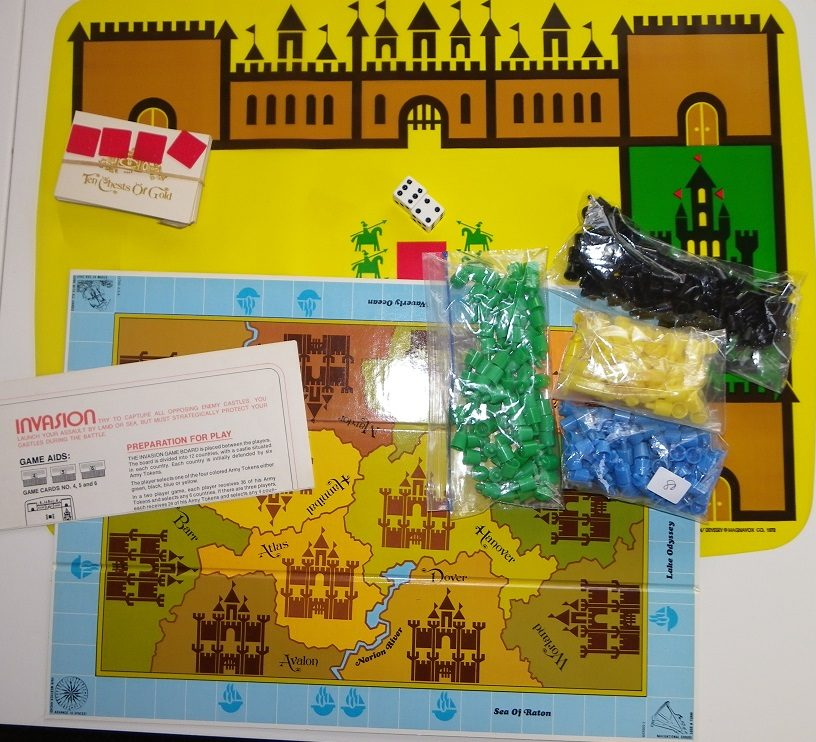
\includegraphics[width=0.45\textwidth]{resources/figures/invasion.jpg}
    \caption{Fyzické komponenty a~nalepovací plán hry \textit{Invasion} \cite{invasion}}
    \label{fig:invasion}
\end{figure}

V~roce 1983 vyšlo hned několik her, které kombinovaly fyzickou hrací desku s~digitálním prostředím. Jednou z~nich byla společností \textit{Epyx} vydaná hra \textit{Oil Barons}. Jednalo se o~počítačovou hru, která byla určena pro zařízení \textit{DOS}, \textit{Apple II} a~\textit{Commodore 64}. Její součástí byla fyzická hrací deska a~několik herních tokenů. Samotný program měl za úkol simulovat náhodné výsledky a~udržovat stav hry. UI této hry bylo jednoduché a~odpovídalo své době, jak lze vidět na Obrázku \ref{fig:oil_barons}. \cite{oil_barons}

\begin{figure}[H]
    \centering
    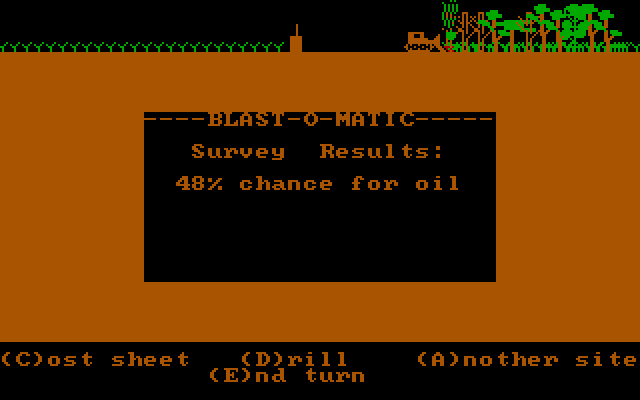
\includegraphics[width=0.45\textwidth]{resources/figures/oil_barons.png}
    \caption{Příklad GUI hry \textit{Oil Barons} \cite{oil_barons}}
    \label{fig:oil_barons}
\end{figure}

Další významný vývoj této kategorie hybridních her se ubíral nejčastěji k~mobilním aplikacím a~takzvaným companion apps (podpůrným aplikacím). Tyto aplikace slouží k~různým účelům, jako je například výběr či správa herních prvků nebo vyprávění příběhu. Většina těchto aplikací je oficiální součástí dané hry a~bez jejího použití není možné ji odehrát. Mezi ně patří například hra \textit{Na vlnách neznáma} (původním názvem \textit{Forgotten Waters}), která využívá aplikaci k~vyprávění příběhu, správě nepřátel a~k~výběru dějové linky.

\subsection{Hry s~rozšířenou realitou}
Nejmladší kategorií hybridních her jsou hry s~rozšířenou realitou (augmented reality, neboli AR). Tyto hry využívají technologie, které umožňují hráčům interagovat s~digitálními prvky ve skutečném světě. První takovou hrou byla \textit{AR Quake}, která byla vytvořena v~roce 2000. Aby si ji hráč mohl vyzkoušet, musel mít nasazený speciální batoh s~počítačem, který pomocí gyroskopů určoval jeho polohu a~promítal obraz digitálního světa přes speciální brýle. Hra byla vytvořena jako experiment, který měl ukázat možnosti AR technologií. \cite{ar_history}

Největší rozvoj v~popularitě AR her nastal až s~vydáním aplikace \textit{Pokémon GO} v~roce 2016. Tato hra využívala GPS a~kameru mobilního telefonu k~tomu, aby hráči ve skutečném světě mohli hledat a~chytat virtuální postavičky. Hra byla velice populární a~stala se tak první AR hrou, která se dostala do povědomí široké veřejnosti.

\section{Vybrané hybridní hry}
Následující hry jsem vybral jako příklady a~inspiraci pro tuto práci. Jedná se o~stolní hry, které nějakým způsobem využívají právě internetových aplikací pro umocnění herního zážitku, organizaci hry či správu herních mechanismů.

\subsection{Na vlnách neznáma}
První z~těchto her je \textit{Na vlnách neznáma}, vydaná v~roce 2020 společností \textit{Plaid Hat Games}. Jedná se o~výpravnou RPG hru, ve které se hráči ujímají rolí pirátů a~společně čelí dobrodružstvím a~nástrahám, jež rozmanitý příběh této hry nabízí. Hra samotná využívá oficiální internetovou aplikaci \cite{forgotten_waters_app}, která slouží k~vyprávění herního děje pomocí namluvených scén a~k~zaznamenávání hráčských rozhodnutí, na kterých závisí dynamický rozvoj příběhu této hry. Aplikace dále udává životy a~statistiky nepřátel, slouží k~výběru kampaně (dějové linky) a~v~neposlední řadě přispívá k~zážitku hráčů pomocí namluvených scén.

Fyzické komponenty hry obsahují herní plán s~hexagonálními políčky a~s~tokeny lokací, které si hráči rozestaví podle pokynů aplikace. Dále obsahuje kartonové figurky, osobní deníky postav, knihu lokací, balíček karet a~sadu kostek. Kartonové figurky s~potiskem v~kombinaci s~osobními deníky, do kterých si hráči zapisují informace, představují postavy. Zároveň se ve hře nachází několik ukazatelů a~počítadel, jež se využívají v~různých aspektech hry. V~knize lokací lze najít popisy míst, které mohou hráči ve hře navštívit, a~zároveň možnosti, jež se jim v~těchto lokacích nabízejí. Karty v~balíčku představují poklady a~úryvky příběhu. Oba tyto druhy přináší hráči buďto pozitivní nebo negativní efekty, které ovlivňují jeho postavu. Sada kostek se využívá k~určování výsledků různých akcí, jež hráči mohou provést.

\subsection{Gloomhaven}
Druhou hrou, kterou bych chtěl uvést, je \textit{Gloomhaven}. Tato hra byla vydána v~roce 2017 společností \textit{Cephalofair Games}. Jde o~kooperativní fantasy hru, ve které se hráči vcítí do role dobrodruhů, jenž se snaží přežít v~nehostinném světě, plnit různé úkoly a~odkrývat příběh, který před nimi leží. Hra je ve stylu dungeon crawl, což znamená, že hlavní náplní hry je postup z~lokace do lokace, kde hráče čekají úkoly a~boj s~nepřáteli. Původně je hra koncipována jako čistě stolní hra, ale kvůli velkému množství fyzických komponent (Obrázek \ref{fig:gloomhaven_contents}), které hra obsahuje, začaly vznikat aplikace, jež mají za úkol organizaci hry usnadnit. Jednou z~nich byla aplikace \textit{Gloomhaven Helper} \cite{gloomhaven_helper}, která se na čas stala i~oficiální aplikací pro tuto hru, avšak kvůli licenčním problémům byla zrušena. Po jejím stažení z trhu vzniklo několik nástupců. Jedním z~nich je \textit{Gloomhaven Secretariat} \cite{gloomhaven_secretariat}, který slouží k~organizaci hry, správě nepřátel i~postav. Také umožňuje hráčům zaznamenávat své postupy v~příběhu, výsledky bitev a~další herní prvky.

\begin{figure}[H]
    \centering
    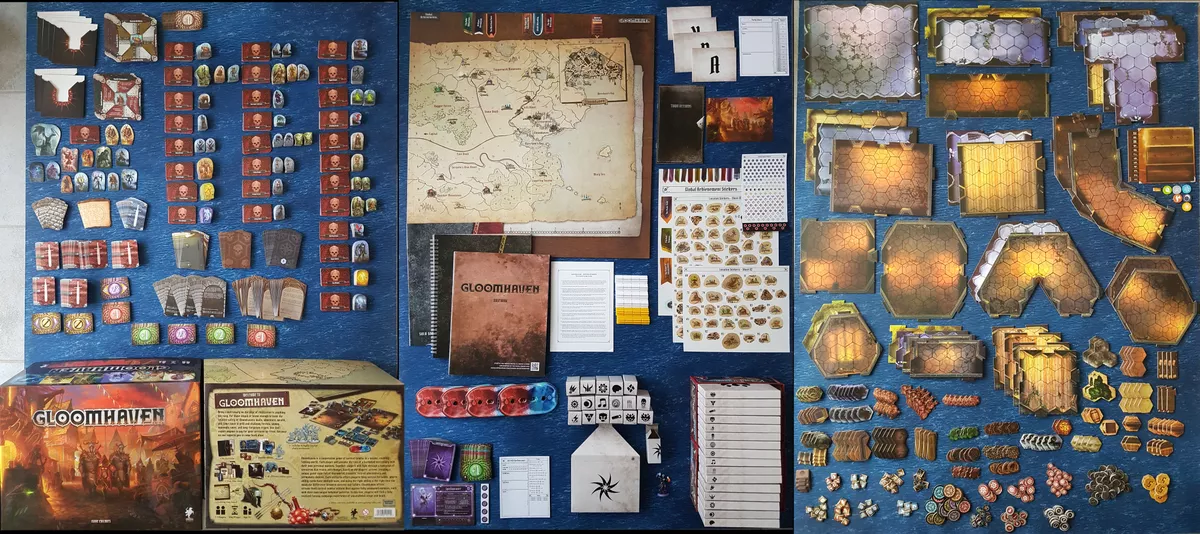
\includegraphics[width=0.9\textwidth]{resources/figures/gloomhaven.png}
    \caption{Fyzické komponenty deskové hry \textit{Gloomhaven} \cite{gloomhaven}}
    \label{fig:gloomhaven_contents}
\end{figure}

Fyzická součást hry obsahuje mapu světa, na kterou hráči postupně přilepují nálepky odemčených lokací a~svých úspěchů. Hra obsahuje díly lokací, což jsou části hrací desky, které lze složit k~sobě. Tyto části jsou potištěny hexagonovou sítí, která slouží jako políčka pro hráčské figurky. Dále se zde nachází kniha lokací, která popisuje příběh a~udává rozložení a~díly potřebné pro složení jednotlivých lokací. Každý typ nepřítele má svou kartu statistik a~vlastní balíček karet, které určují jeho chování a~možné akce. Pro všechny nepřátele existuje jeden společný balíček modifikátorů (karet, které namísto kostek slouží k~vytváření nahodilých výsledků). Podobně má každá postava také svou sadu karet akcí a~velkou kartu statistik, zároveň má však každý hráč vlastní balíček modifikátorů a~počítadlo životů. Figurky postav jsou vyrobeny z~plastu a~jsou velice detailní. Kartonové figurky s~plastovými stojánky představují nepřátele. Dále hra obsahuje velké množství kartiček předmětů, které hráči mohou používat, tokeny peněz, poškození a~efektů.
\chapter{Uživatelské rozhraní}

\section{Stručná historie GUI}
Počátek grafických rozhraní se datuje do osmdesátých let minulého století, kdy firma Xerox vyvinula počítač Alto. Jednalo se o první počítač, jehož rozhraní se skládalo z oken, ikon a používalo myš k ovládání. Toto grafické rozhraní pak posloužilo jako odrazový můstek a základ dalším projektům. Jeden z nich byl například Apple Macintosh, který grafické uživatelské rozhraní popularizoval. Dále přišel operační systém Windows, který GUI posunul ještě dál mezi mainstreamové uživatele. GUI se postupem let vyvíjelo společně s novými technologiemi a nyní je neoddělitelnou součástí téměř všech počítačových systémů.

\section{Zásady vývoje webového GUI}
Následující zásady jsou základem přívětivého UI, ve kterém se dokáže uživateů snadno orientovat a které je příjemné na pohled. Vychází z praktických zkušeností grafiků i psychologických poznatků. 

% \subsection{Vzhled}
\subsection{Obecné zásady}
Následující text se věnuje nejzákladnějším principům, které by mělo uživatelské rozhraní splňovat.\cite{principles_of_design}

\subsubsection*{Kontrast}
Kontrast je jedním z nejdůležitějších prvků designu. Zajišťuje, že text a další prvky jsou čitelné a viditelné. Je důležitý pro umocnění dojmu a pro zvýraznění důležitých prvků.

\subsubsection*{Balanc}
Všechny prvky na stránce mají pomyslou váhu, která je dána jejich velikostí, barvou, kontrastem a dalšími faktory. Zajišťuje, že tyto prvky jsou rozloženy tak, aby stránka působila vyváženě a přehledně.

\subsubsection*{Důraz}
Důraz slouží pro zvýraznění důležitých prvků a k pomyslnénu ukrytí těch méně podstatných. Můžeme tak ovládat výraznost jistých informací a zároveň usměrňovat pozornost uživatele.

\subsubsection*{Proporce}
Správně určené proporce podporují výše zmíněný balanc. Pomáhají uživateli orientovat se na stránce a zároveň zajišťují, že stránka působí přehledně a esteticky.

\subsubsection*{Hierarchie}
Hierarchie je v designu klíčová, zejména pokud jde o zdůraznění důležitých prvků. Tento princip je často demonstrován prostřednictvím titulů a nadpisů. Titul stránky by měl okamžitě vyniknout jako nejdůležitější prvek, zatímco nadpisy by měly být formátovány tak, aby naznačovaly svůj význam ve vztahu k sobě navzájem a k obsahu, který uvádějí.

\subsubsection*{Opakování}
Opakování je účinným nástrojem pro zdůraznění a sjednocení myšlenek v rámci designu. Lze ho dosáhnout konzistentním použitím barev, písem, tvarů nebo jiných prvků designu. Konzistentní formátování pomáhá sjednotit prvky na celé stránce.

\subsubsection*{Rytmus}
Slovem rytmus je myšlen styl, jakým jsou prvky (ať už mezery, barvy, velikosti, atd.) na stránce uspořádány a v jakém pořadí použity. Některé rytmické vzory mohou vzbuzovat pocit uspořádanosti a přehlednosti, zatímco jiné mohou působit chaoticky.

\subsubsection*{Vzor}
V uživateli vzory vyvolávají pocit předvídatelnosti a pohodlí. Může se jednat například o rozložení stránky, které se běžně používá, nebo o způsob zadávání dat, který je uživatelům známý.

\subsubsection*{Volný prostor}
Volný prostor (white space) je prázdný prostor mezi prvky na stránce, který pomáhá zvýraznit důležité prvky a zároveň zajišťuje, že stránka není přeplněná.

\subsubsection*{Pohyb zraku po stránce}
Tohoto principu lze dosáhnout dodržením výše zmíněných prvků. Jde o kombinaci všech předešlých principů a jejich aplikaci tak, aby uživatel mohl snadno a pohodlně stránku použít.

\subsubsection*{Rozmanitost}
Na rozdíl od předešlých bodů, rozmanitost nenapomáhá orientaci na stránce, ale zajišťuje, aby byla pro uživatele zajímavá.

\subsubsection*{Spojitost}
Spojitost zajišťuje, že všechny prvky na stránce působí jako celek. Většinou se jedná o opakování barev, či používání minimálního množství fontů.

% \begin{itemize}
%     \item \textbf{Kontrast}: Zajišťuje, že text a další prvky jsou čitelné a viditelné.
%     \item \textbf{Balanc}: Udržuje vyváženost prvků na stránce.
%     \item \textbf{Důraz}: Zvýrazňuje důležité prvky a pomáhá usměrňovat pozornost uživatele.
%     \item \textbf{Proporce}: Podporují balanc a pomáhají uživateli orientovat se na stránce.
%     \item \textbf{Hierarchie}: Důležitá pro zdůraznění prvků, zvláště titulů a nadpisů.
%     \item \textbf{Opakování}: Slouží k sjednocení myšlenek v rámci designu.
%     \item \textbf{Rytmus}: Určuje uspořádání prvků na stránce, což může vyvolat pocit přehlednosti.
%     \item \textbf{Vzor}: Vybuzuje pocit předvídatelnosti a pohodlí.
%     \item \textbf{Volný prostor}: Pomáhá zvýraznit důležité prvky a udržuje stránku přehlednou.
%     \item \textbf{Pohyb zraku po stránce}: Pořadí v jakém si uživatel prvků všimne. Zajišťuje to kombinace předešlých principů.
%     \item \textbf{Rozmanitost}: Zajišťuje, aby stránka byla zajímavá pro uživatele.
%     \item \textbf{Spojitost}: Zajišťuje, že všechny prvky působí jako celek.
% \end{itemize}

\subsection{Teorie barev}
Výběr barev je nedílnou součástí vývoje každého GUI. Teorie barev se zabývá vztahy mezi barvami a jejich významem. Poznáním těchto nuancí může vývojář využít barvy k ovlivnění uživatelova vnímání své aplikace. Různé barvy mohou budit různý psychologický a emocioální význam. Teorie barev poskytuje základní pravidla a směrnice pro efektivní použití barev v designu, aby se dosáhlo esteticky příjemného výsledku a vyvolalo se požadované emoční nebo vizuální působení. Teorie barev také udává, že existuje několik kategorií základních barev:
\begin{itemize}
    \item \textbf{Primární barvy}: Červená, modrá a žlutá. Tyto barvy nelze vytvořit kombinací jiných barev.
    \item \textbf{Sekundární barvy}: Zelená, fialová a oranžová. Tyto barvy vzniknou smícháním dvou primárních barev.
    \item \textbf{Terciární barvy}: Těchto šest barev vznikne smícháním primárních a sekundárních barvev. Patří sem například růžová, tyrkysová, či žlutozelená.
\end{itemize}

Těchto dvanáct barev samozřejmě není jedinými barvami, které lze zejména v počítačové grafice použít. Díky tomu se začalo v grafice používat takzvaný color wheel (barevný kruh).\cite{color_theory_design}

\subsubsection{Color wheel}
Barevný kruh se často používá díky jeho intuitivnímu rozložení barev. Obsahuje všechny barvy, které lze vytvořit smícháním tří primárních barev a díky přidání černé, či bílé barvy umožňuje i úpravu jejich odstínů. Existuje několik způsobů, jak za pomoci tohoto kruhu vybrat:
\begin{itemize}
    \item \textbf{Komplementární}: Barvy, které jsou na opačných stranách kruhu. Při jejich kombinaci vzniká kontrastní efekt.
    \item \textbf{Monochromatické}: Tyto barvy je sada odstínů jedné barvy. Vytváří harmonický efekt.
    \item \textbf{Analogické}: Barvy, které jsou vedle sebe na kruhu. Vytváří přirozený a pohodlný efekt, ale je vhodné vybrat jednu z barev jako hlavní a zbytek používat pouze jako akcenty.
    \item \textbf{Triadické}: Kombinace tří barev, které na kruhu tvoří rovnostranný trojúhelník. Podobně jako způsob komplementární, také vytváří kontrastní efekt.
    \item \textbf{Tetradické}: Čtyři barvy, které jsou od sebe na kruhu položeny stejně daleko. Vytváří podobný efekt jako triadický způsob, ale je těžší je správně kombinovat.
\end{itemize}\cite{color_wheel}

% \subsection{Použitelnost}

\section{GUI ve vybraných hybridních hrách}

\subsection{Na vlnách neznáma}
Aplikace pro hru Na vlnách neznáma je primárně zamýšlená pro mobilní zařízení, čemuž odpovídá její design. Jedná se o responzivní jednostránkovou aplikaci. Samotná stránka obsahuje základní nastavení přístupnosti a jazyka, informace o aplikaci samotné a především možnost hru spustit. Po spuštění zůstane na stránce pouze jednoduchý vstup pro číslo, které představuje záznam, jenž má aplikace zobrazit. Vždy je možné otevřít historii předešlých záznamů, náhled mapy a časovač. Při načtení záznamu se zobrazí možnosti, které nabízí, a stránka spustí naraci příběhu, který je v něm obsažen. Samotná aplikace je velmi jednoduchá a přímočará, takže představuje ideální doprovod k samotné hře. Věnuje také velkou pozornost přívětivé grafice, což také napomáhá imerzi.


\subsection{Gloomhaven}
Gloomhaven Secretariat je jedna z aplikací pro hru Gloomhaven, která se stará o její největší část, a to souboje. Opět se jedná o jednostránkovou webovou aplikaci. Stránka je primárně určena pro desktop, či jiná zařízení s velkou obrazovkou. Je sice použitelná i na mobilních zařízeních, ale jedná se pouze o zmenšenou verzi klasické stránky bez dalších úprav. To znamená, že některá tlačítka jsou příliš malá pro pohodlné používání. Obsah se také zdá být poměrné jednoduchý, avšak už není tak intuitivní, jako u předešlého příkladu. Po otevření stránky se zobrazí spousta informací a novému uživateli se tak může snadno stát, že se v nich ztratí. Po spuštění aplikace hráče mimo jiné vyzve k výběru příběhové linie, kterou chtějí začít a následně k přidání postav. Stránka pak nabízí spoustu možností, které jsou uživateli k dispozici, ale k žádné z nich nedodá hlubší vysvětlení. Stránka potřebuje neustálé vstupy, aby plnila svou funkci, ty jsou však také někdy neintuitivní a jejich zadávání zdlouhavé.

\section{Volba technologií pro vývoj GUI}
Zprvopočátku jsem vytvořil prototyp GUI v čistém HTML a CSS, abych věděl, jak bude samotný produkt zhruba vypadat. Poté jsem svou pozornost obrátil na výběr technologií, které budu pro vývoj GUI používat. Hlavními kandidáty byly frameworky React, Angular a Svelte.

\subsection{Frameworky}

\subsubsection{React}
React je jednou z nejpopulárnějších moderních platforem pro tvorbu webových aplikací. Je to open-source JavaScript knihovna vyvinutá a udržovaná společností Meta (bývalý Facebook). Používá deklarativní programovací paradigma, což znamená, že vývojář specifikuje, jak by měl výsledek vypadat, bez toho, aby musel explicitně popsat, jak daného výsledku dosáhnout. Zároveň je založen na komponentovém přístupu -- celý kód je rozdělen do menších celků zvaných komponenty, což je kombinace JS a HTML, které jsou modulární a znovupoužitelné. Díky jeho schopnosti aktualizovat jednotlivé komponenty se nejčastěji používá pro vývoj jednostránkových webových aplikací. React je známý svou komunitou a ekosystémem, který je kolem něj postavený. Díky tomu je možné najít spoustu předpřipravených komponent a knihoven, které urychlí vývoj aplikace. Zároveň má však poměrně strmou křivku učení, což z něj dělá nepřívětivou volbu pro začátečníky.

React využívá virtuální DOM, který zajišťuje rychlejší a efektivnější vykreslování změn. Při změně v komponentě se nevykreslí celá stránka, ale pouze upravená část. Tím se značně zrychlí vykreslování a zároveň sníží nároky na výkon.\cite{react, what_react_is_and_why_it_matters,angular_vs_react}

\subsubsection{Angular}
Angular je další z vysoce populárních frameworků pro vývoj UI. Opět se jedná o open-source platformu, nyní však vyvinutou a udržovanou společností Google. Angular je založen na jazyce TypeScript a stejně jako React využívá komponentového přístupu a deklarativního programovacího paradigmatu. Jeho převážný význam spočívá ve vytváření rozsáhlých dynamických webových aplikací. Na rozdíl od Reactu se jedná o plněhodnotný framework, který používá reálný DOM. Samotný framework je robustní a bezpečný, což z něj dělá ideální volbu pro vývoj aplikací, které pracují s citlivými daty. Na druhou stranu je však poměrně složitý a náročný na výkon, což je pro menší aplikace nevhodné.\cite{what_is_angular,angular_vs_react}

\subsubsection{Svelte}
Svelte je moderní framework pro tvorbu webových aplikací. Jedná se o open-source software vyvinutý Richem Harrisem. Svelte se od ostatních frameworků liší tím, že se jeho kód při buildu převede na čistý optimalizovaný JavaScript. Tím se výsledná aplikace značně zrychlí a zároveň se sníží nároky na výkon na straně uživatele. Svelte také nabízí velmi jednoduchý a přívětivý způsob psaní kódu, který vývoj aplikace urychlí. Dokáže také pracovat s TypeScript soubory bez nutnosti jejich předešlé kompilace, což výsledný kód dělá mnohem bezpečnějším a přehlednějším.\cite{svelte_and_why_you_should_consider_it,svelte}

\subsubsection{Srovnání}
Vzhledem k tomu, že projekt obnáší vytvořiení GUI pro hybridní stolní hru, která nebude nijak extrémně rozsáhlá, a zároveň bude potřebovat co největší rychlost a efektivitu, byl nakoinec vybrán framework Svelte. Ten nabízí všechny potřebné funkce a zároveň je velmi rychlý a efektivní. Jeho jednoduchost by také měla přispět k rychlejšímu vývoji bez dalších větších problémů.

\subsection{Další technologie}
Dále jsem se rozhodl používat CSS knihovny, které dokáží ušetřit práci s designem a responzivitou a zároveň zrychlí vývoj aplikace. Jako hlavní kandidáti se ukázaly Bootstrap a Tailwind CSS. Bootstrap je velmi populární knihovna, která nabízí spoustu předpřipravených komponent a stylů. Tailwind CSS je naopak známý svou flexibilitou a možnostmi přizpůsobení.
***V plánu rozepsat.***

\chapter{Návrh herního systému}
\label{chap:design}

Na základě požadavků stanovených v předchozí kapitole \chapterref{chap:requirements} byl vytvořen návrh herního systému, který je pro přehlednost rozdělen do několika částí. První část se zabývá návrhem herních modelů, druhá se zaměřuje na herní mechaniky a třetí popisuje návrh herních komponent.


\section{Schéma hry}
\label{sec:design_scheme}

Na návrhu databáze pracoval celý tým vyvíjející modelovou hru, jak je popsáno v \customref{Kapitole}{subsec:database}, její rozvržení je však skvělým nástrojem pro popsání návrhu herních modelů, proto bude detailně rozebráno v následující kapitole.

\begin{figure}[h]
    \centering
    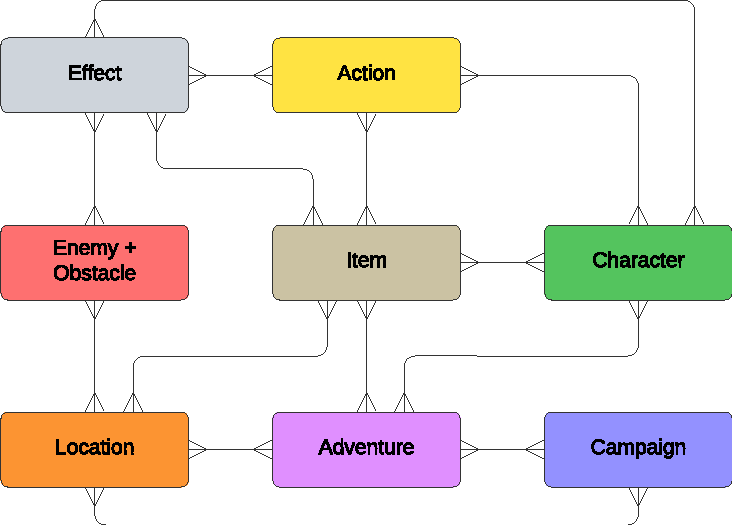
\includegraphics[scale=0.95]{../../shared/diagrams/er_macro.pdf}
    \caption{Makro pohled na schéma databáze}
    \label{diag:er_macro}
\end{figure}

Na \customref{Obrázku}{diag:er_macro} je orientačně zobrazen makro pohled na schéma databáze, které je pro přehlednost rozděleno do několika barevně rozlišených částí, neboť celková databáze zahrnuje 45 tabulek. Každá z těchto částí je následně podrobněji popsána v následujících kapitolách. Celkové schéma databáze je zobrazeno v \customref{Příloze}{chap:database_schema}.


\subsection{Akce}
\label{subsec:schema_actions}

Popis celkového rozvržení herních komponent začíná \customref{Obrázkem}{diag:er_action}, který definuje strukturu \textbf{akcí} \attr{Action}, jejichž mechanická funkcionalita je dále rozepsána v \customref{Kapitole}{subsec:design_actions}. Každá akce má svůj název \attr{title} a popis \attr{description}, který hráči pomůže pochopit, co daná akce přibližně znamená, bez nutnosti hlubšího studia samotné karty. Dále je v akci uchována informace o jejím zahození \attr{discard}, která určuje, v jakém případě a na jak dlouho musí hráč po odehrání danou kartu zahodit. Každá akce má také požadovanou úroveň \attr{levelReq}, která umožňuje tvorbu akcí, které hráči mohou odemykat spolu s postupem příběhem.

\begin{figure}[h]
    \centering
    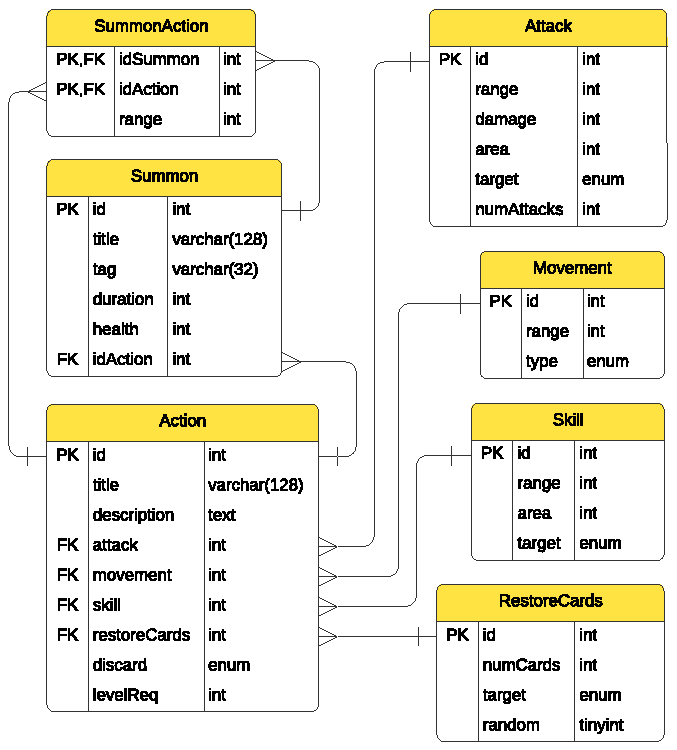
\includegraphics{../../shared/diagrams/er_action.pdf}
    \caption{Schéma akcí}
    \label{diag:er_action}
\end{figure}

V modelové hře se akce skládají z pěti částí, interně nazývanými \textit{features} neboli \textit{prvky akce}. Jedná se o \textit{pohyb} \attr{Movement}, \textit{útok} \attr{Attack}, \textit{schopnost} \attr{Skill}, \textit{poskok} \attr{Summon} a \textit{obnovení karet} \attr{RestoreCards}. Každý z prvků je nepovinný a může být v akci využit maximálně jednou s výjimkou poskoků, kterých může jedna akce vyvolat libovolný počet. Samotní poskoci poté také mají svou vlastní akci, kterou ve svém kole konají. Průběh jednotlivých prvků je popsán v \customref{Kapitole}{subsec:design_actions}.


\subsection{Postavy}
\label{subsec:schema_character}

Na \customref{Obrázku}{diag:er_character} je zobrazeno schéma nejen postav, ale i předmětů, neboť jsou k sobě úzce vázány. 

\begin{figure}[h]
    \centering
    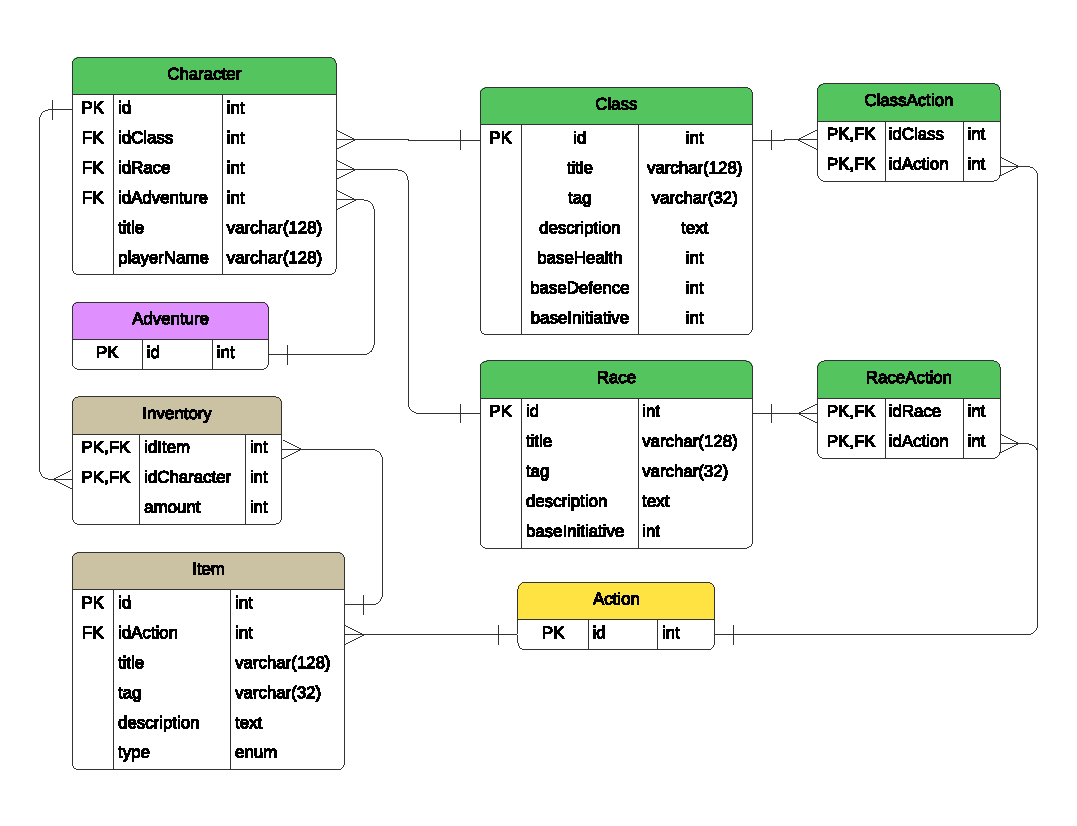
\includegraphics[width=\textwidth]{../../shared/diagrams/er_character.pdf}
    \caption{Schéma postav}
    \label{diag:er_character}
\end{figure}

\textbf{Postava} \attr{Character} má několik základních vlastností, které ji definují -- jméno postavy \attr{title} a jméno hráče \attr{playerName}, dále je však každá postava složena z kombinace \textbf{rasy} \attr{Race} a \textbf{třídy} \attr{Class}. Obě tyto tabulky obsahují jméno \attr{title}, popis \attr{description} a štítek \attr{tag}, který slouží k identifikaci obrázku, který jim přísluší. U obou je také zaznamenána základní iniciativa, třída však obsahuje také definici základního zdraví a obrany postavy. Postava je vždy vázána na jedno určité dobrodružství.

Každá postava může mít také vybavení, které je k ní navázáno přes \textbf{inventář} \attr{Inventory}, kde se zaznamenává, kolik kterého typu předmětu postava má. Samotné \textbf{předměty} \attr{Item} jsou podobně jako rasy a třídy složeny z názvu, popisu a štítku, kromě toho však také obsahují informaci o jejich typu \attr{type}, který určuje, zda se jedná o zbraň, brnění nebo jiný typ předmětu.

Předměty, rasy a třídy mohou být chápány jako možnosti získání určitých akcí, neboť všechny tři tabulky mají na akce vazbu. Rasa a třída může hráči poskytovat neomezené množství akcí, předmět však má vždy jen jednu akci, kterou hráč může využít, což je limitace zavedená z důvodu přehlednosti fyzických komponent, popsaných v \customref{Kapitole}{subsec:design_cards}.

\subsection{Lokace}
\label{subsec:schema_location}

Schéma lokací zobrazeno na \customref{Obrázku}{diag:er_location} je díky velkému množství složených primárních klíčů složené z mnoha vazeb, i přes jejich četnost však není nijak zvlášť komplikované.

\begin{figure}[h]
    \centering
    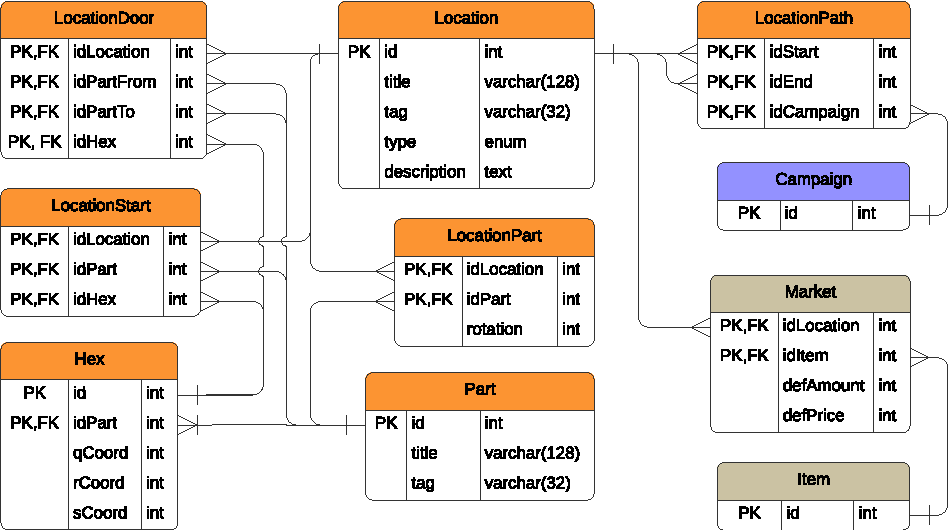
\includegraphics{../../shared/diagrams/er_location.pdf}
    \caption{Schéma lokací}
    \label{diag:er_location}
\end{figure}

\textbf{Lokace} \attr{Location} je základním prvkem hry, který hráči umožňuje prozkoumávat herní svět. Ve své podstatě se jedná o místo na herní mapě, které hráči mohou navštívit. Každá lokace má své jméno \attr{title}, popis \attr{description} a štítek \attr{tag}, podobně jako předchozí entity. Dále si nese informaci o typu \attr{type}, jenž určuje, zda se jedná o lokaci se soubojem \attr{encounter} nebo o obchod \attr{market}, nejčastěji se však používá první možnost, pro kterou se poté využívají ostatní tabulky pro zápis herní plochy.

Každá lokace se skládá z několika \textbf{částí} mapy \attr{Part}, které mohou být na stole různě otočené, proto je jejich rotace \attr{rotation} také zaznamenaná. Části mají opět nejen jméno ale i štítek, který má tentokrát ještě další funkcionalitu, neboť představuje identifikátor, který umožňuje hráčům snadno najít odpovídající části mapy mezi ostatními herními komponentami. Herní pole je dále rozděleno na \textbf{hexagony}, u kterých bylo rozhodnuto o použití tzv. kubického souřadného systému, který polím ve 2D prostoru přiřadí 3D souřadnice (\texttt{q}, \texttt{r}, \texttt{s}), což usnadňuje výpočty pro herní mechaniky, které se týkají pohybu a vzdáleností mezi jednotlivými políčky.

Jak jde vidět z \customref{Obrázku}{diag:er_location}, lokace jsou spolu s ostatními tabulkami propojeny spoustou vazeb, které umožňují hlubší specifikaci propojení. Jedná se například o reprezentaci dveří spojující části herní desky v rámci lokace \attr{LocationDoor}, počáteční políčka lokace, kde se na začátku souboje umisťují postavy hráčů \attr{LocationStart}, nebo propojení s kampaní, v rámci které jsou na sebe lokace dynamicky navázány ve světové mapě \attr{LocationPath}. Speciálním případem vazební tabulky je pak obchod \attr{Market}, který pro danou lokaci určuje nabízené předměty, jejich množství a ceny.

\subsubsection*{Nepřátelé a překážky}
\label{subsubsec:schema_enemy_obstacle}

Lokace jsou zaplněny nepřáteli \attr{Enemy} a překážkami \attr{Obstacle}, jak je možné vyčíst z \customref{Obrázku}{diag:er_enemy_obstacle}. Obě dvě entity opět obsahují informace o názvu, popisu a štítku pro vyhledávání obrázků a také mají vazbu na hexagon neboli políčko určité lokace, na kterém se vyskytují (\texttt{HexEnemy} a \texttt{HexObstacle}), dále se však mírně liší.

\begin{figure}[h]
    \centering
    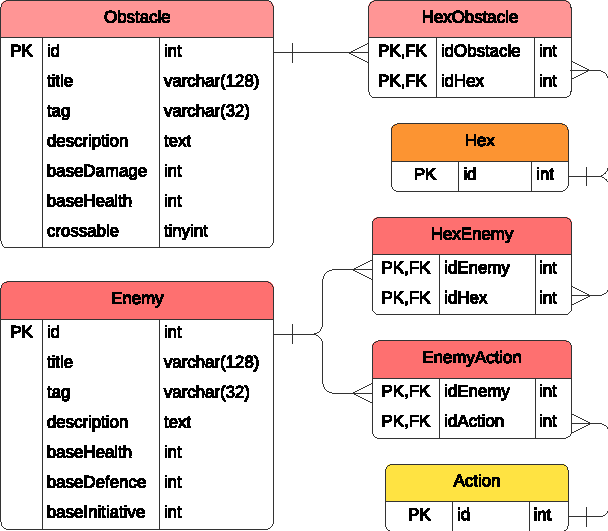
\includegraphics{../../shared/diagrams/er_enemy_obstacle.pdf}
    \caption{Schéma nepřátel a překážek}
    \label{diag:er_enemy_obstacle}
\end{figure}

\textbf{Nepřátelé} v podstatě kopírují statistiky postav, mají své vlastní zdraví, obranu a iniciativu. Dále také mohou mít své vlastní akce, které budou v souboji provádět \attr{EnemyAction}.

\textbf{Překážky} jsou oproti nim pasivní, proto mají zaznamenané pouze své zdraví a míru zranění, které dostane entita, která se na ní zraní. Také má indikátor toho, zda je tato překážka průchozí \attr{crossable} nebo nikoliv.


\subsection{Kampaň}
\label{subsec:schema_campaign}

Kampaň slouží k reprezentaci celého příběhu, kterým si hráči budou v rámci modelové hry procházet. Její schéma je vyobrazeno na \customref{Obrázku}{diag:er_campaign}.

\begin{figure}[h]
    \centering
    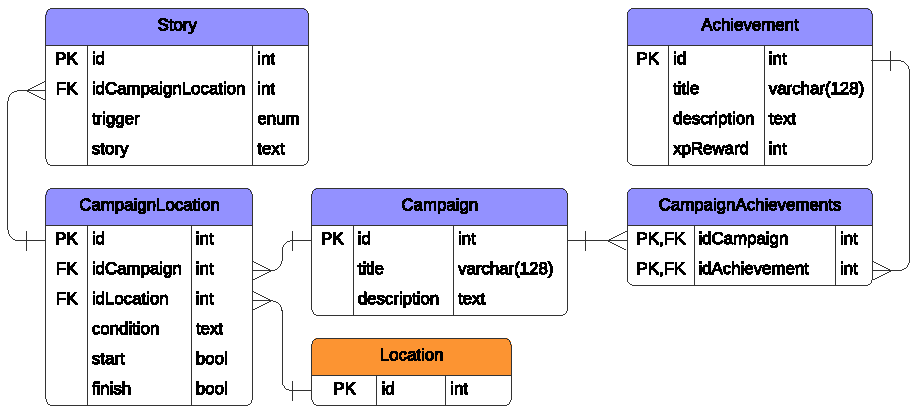
\includegraphics[scale=0.8]{../../shared/diagrams/er_campaign.pdf}
    \caption{Schéma kampaně}
    \label{diag:er_campaign}
\end{figure}

Samotná \textbf{kampaň} \attr{Campaign} si moc dat nenese, obsahuje pouze název a popis. Klíčová je však především její vazba na lokace \attr{CampaignLocation}, které jsou v rámci kampaně propojeny do světové mapy. Tato vazební tabulka obsahuje informace o tom, jaké lokace jsou v rámci kampaně dostupné, zda se jedná o počáteční \attr{start} nebo případně konečnou \attr{finish} lokaci daného příběhu a také jaké jsou podmínky pro dokončení či selhání lokace \attr{condition}. K této vazbě se také připojuje příběh \attr{Story}, který se může spouštět po určitých událostech odehraných v rámci lokace.

Za zmínku také stojí herní \textbf{úspěchy} \attr{Achievement}, které jsou taktéž navázány na kampaň. Jedná se o určité cíle, které hráči mohou splnit v rámci hry a za jejichž dokončení získají odměnu. Tento cíl si vždy nese název, krátký popis a také odměnu v podobě zkušeností.


\subsubsection*{Dobrodružství}
\label{subsubsec:schema_adventure}

Rozehranou kampaň, ve které již hráči dělají příběhový postup, reprezentuje tzv. \textbf{dobrodružství} \attr{Adventure}, které je zobrazeno na \customref{Obrázku}{diag:er_adventure}.

\begin{figure}[h]
    \centering
    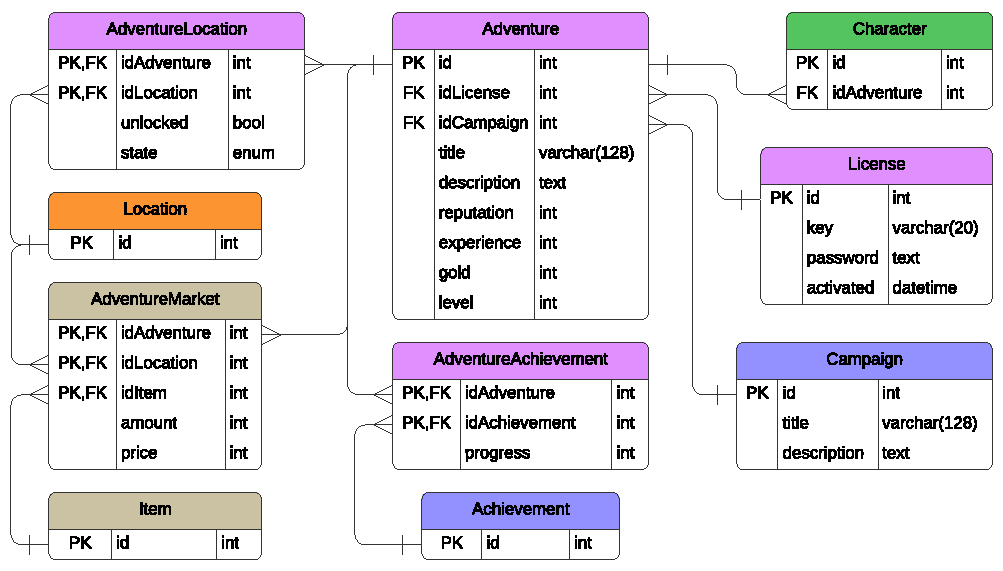
\includegraphics[scale=0.8]{../../shared/diagrams/er_adventure.pdf}
    \caption{Schéma dobrodružství}
    \label{diag:er_adventure}
\end{figure}

Samotná tabulka dobrodružství je relativně objemná, obsahuje kromě klasického názvu a popisu také statistiky rozehrané kampaně, jako je reputace \attr{reputation}, zkušenosti \attr{experience}, peníze \attr{gold} a také úroveň družiny \attr{level}. Úspěchy určité kampaně \attr{AdventureAchievement} se zde taktéž uchovávají spolu s číslem určující postup k danému cíli \attr{progress}.

Vazba na lokace \attr{AdventureLocation} v sobě drží informace o tom, které již byly odemčeny \attr{unlocked} a v jakém stavu \attr{state} jsou, ať už dokončené nebo zatím neúspěšné. Pro podporu dynamičnosti herního rozvoje je zde také možnost upravovat zásoby a ceny v obchodech \attr{AdventureMarket}, které jsou dále vázány na samotné předměty.

Jak již bylo řečeno výše, dobrodružství se může účastnit několik postav. Kromě toho má však dobrodružství nastavenou i \textbf{licenci} \attr{License}, se kterou ho je možné spustit \attr{AdventureLicense}. Licenční klíče jsou náhodně generovaná sekvence dvaceti znaků, které budou distribuovány spolu se hrou a umožní hráčům přistupovat ke svému hernímu účtu a případně si změnit heslo, pomocí kterého se budou do systému přihlašovat. Takto bude zajištěno, že hráči mají přístup pouze na své postavy a příběhy a zároveň se znemožní nelegální kopírování hry.


\subsection{Efekty}
\label{subsec:schema_effect}

Posledním prvkem, který je nutné zmínit, jsou \textbf{efekty} \attr{Effect}, popsány na \customref{Obrázku}{diag:er_effect}. Neboť prolínají celou strukturu hry, nebyly zapsány do jednotlivých grafů výše, ale všechny jejich vazby byly zahrnuty na tomto schématu. 

\begin{figure}[h]
    \centering
    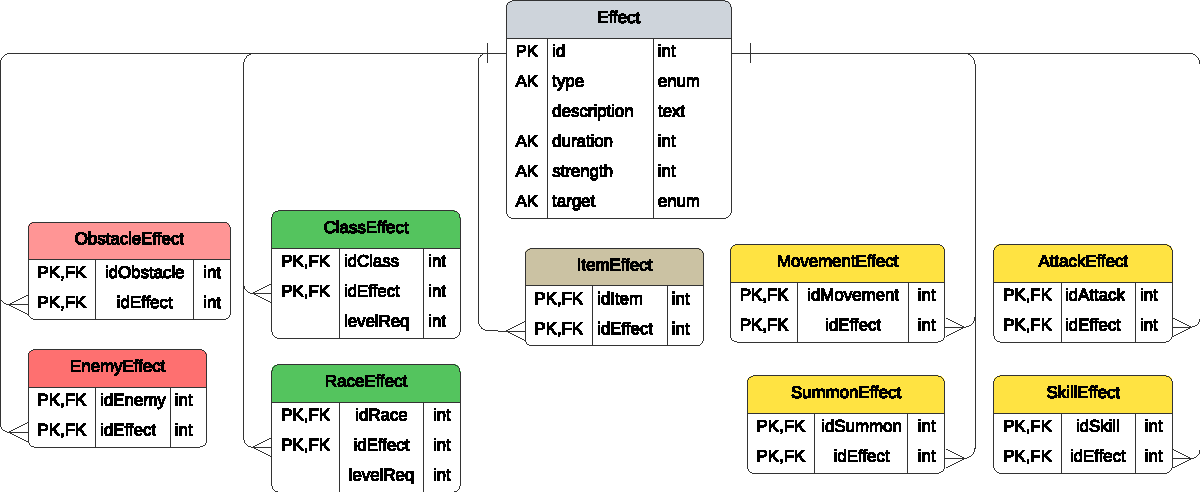
\includegraphics[width=\textwidth]{../../shared/diagrams/er_effect.pdf}
    \caption{Schéma efektů}
    \label{diag:er_effect}
\end{figure}

Hlavní charakteristikou efektu je typ \attr{type}, jejichž mechanická implementace je popsána v \customref{Kapitole}{subsec:design_effects}. Je zde také možnost hráčům předložit popis efektu \attr{description}, který jim pomůže pochopit, co daný efekt znamená. Dále se zaznamenává síla a trvání efektu a také cíl, na který efekt míří.

Efekty mohou být aplikovány na překážky, nepřátele, třídy a rasy, předměty a většinu prvků akce -- pohyb, útok a schopnost. U rasy a třídy je navíc přidán atribut minimální úrovně \attr{levelReq}, který umožňuje postavám odemykat nové pasivní efekty s rostoucí úrovní.


\section{Herní mechaniky}
\label{sec:design_mechanics}

Mechaniky modelové hry jsou silně inspirované především výše zmíněnou deskovou hrou \glsref{gloomhaven}, ale jsou upravené tak, aby lépe vyhovovaly stanoveným požadavkům.


\subsection{Souboj}
\label{subsec:design_encounter}

Souboj je hlavní funkcionalitou, kterou hra nabízí. Průběh souboje je rozdělen do několika fází, které jsou znázorněny na \customref{Obrázku}{diag:encounter}. Ještě před samotným hraním si systém zaznačí, že lokace už byla navštívena (\texttt{visited}), pokud již nemá nastavený jiný stav, který je důležitější (jako například \texttt{completed} nebo \texttt{failed}). Následně hráčům zobrazí příběh, který je s touto lokací spojený.

Poté následuje fáze přípravy hrací desky. Systém zobrazí počáteční místnost lokace, všechny nepřátele, překážky a dveře, které se v ní vyskytují spolu s identifikátory, které umožní hráčům tyto části jednoduše najít a sestavit tak odpovídající konfiguraci místnosti na herním stole. Když je všechno připraveno, hráči umístí své postavy na políčka určená pro hráče a s tím je příprava herního pole hotová.

\newpage
\begin{figure}[H]
    \centering
    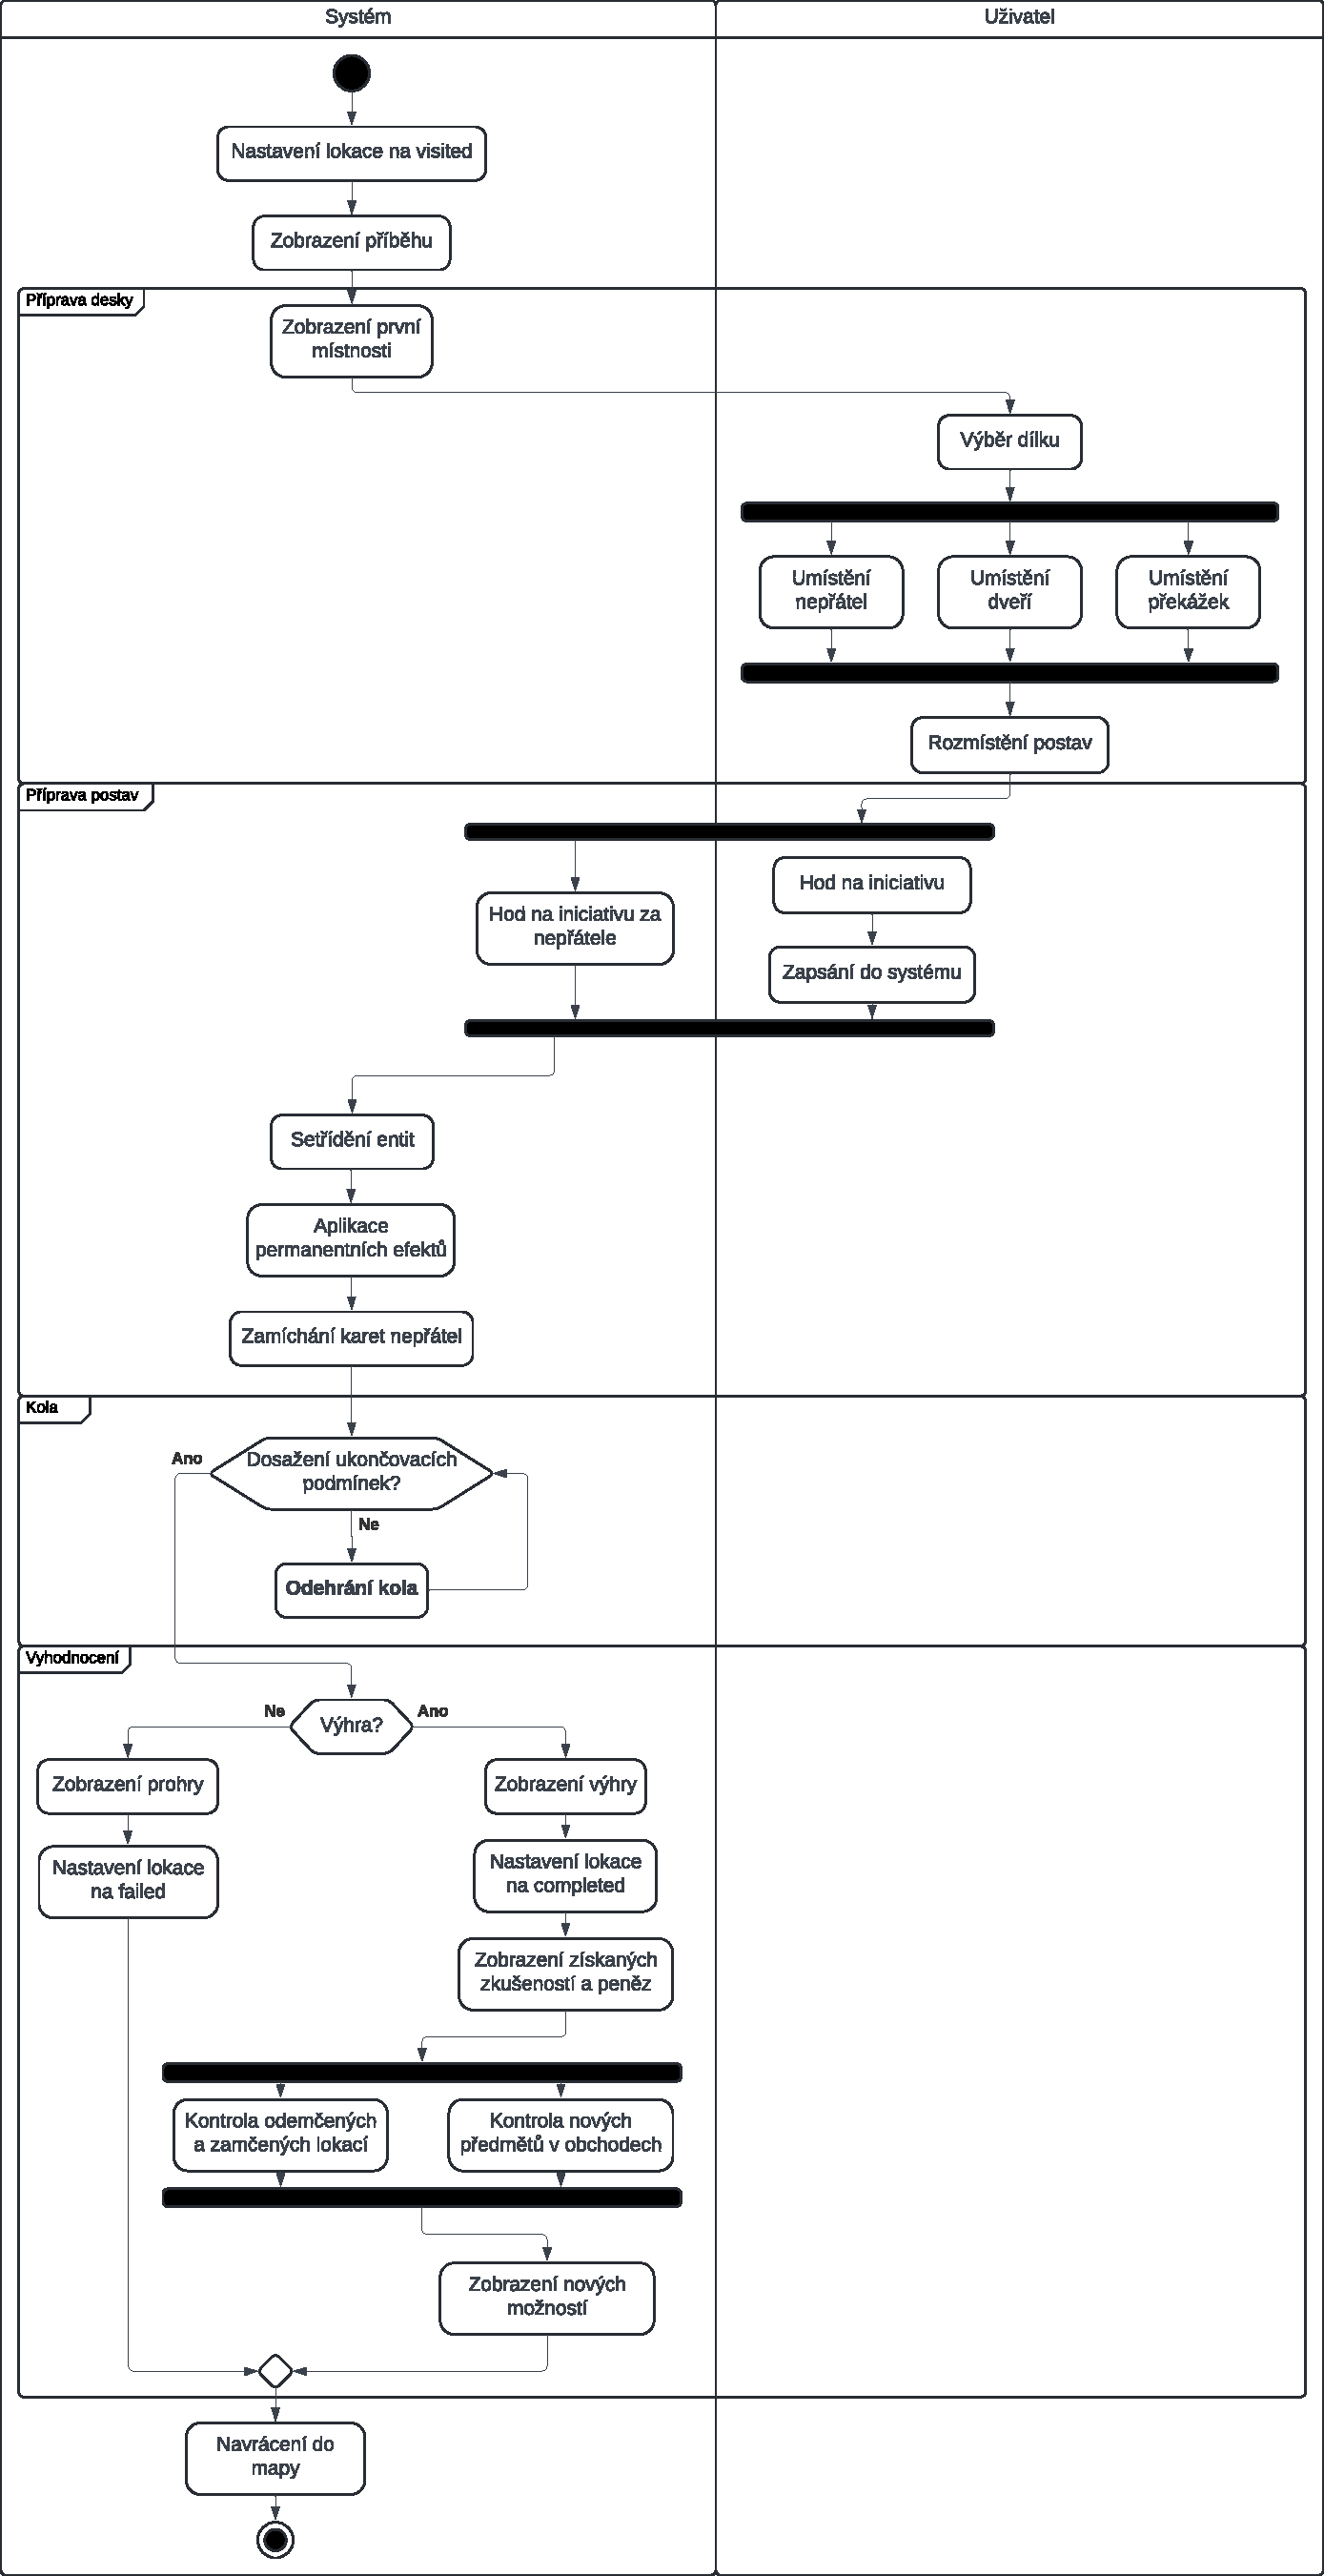
\includegraphics[height=0.98\textheight]{figures/diagrams/encounter.pdf}
    \caption{Diagram průchodu lokací}
    \label{diag:encounter}
\end{figure}
\newpage

Druhá část přípravy je věnována samotným postavám a nepřátelům a tvorbě iniciativního žebříčku. Každý z hráčů si hodí svou kostkou na iniciativu a zaznamená výsledek do systému, který tento modifikátor automaticky přičte k základní výši iniciativy, který hráčova postava získala ze své rasy, třídy a vybavení. Za nepřátele toto provede systém automaticky. Výsledný žebříček je seřazen sestupně a hráči a nepřátelé se podle něj střídají v rámci kola. Dále se tu také provádí aplikace permanentních efektů, tedy efektů získaných ze zázemí a předmětů u postav nebo vrozené efekty u nepřátel, podle \customref{Obrázku}{diag:apply_effect}. Systém pak ještě zamíchá simulovaný balíček nepřátelských karet, který bude sloužit k určení jejich akcí.

Následuje fáze kol, která se provádí podle \customref{Obrázku}{diag:round} opakovaně ve smyčce, dokud hráči nesplní jistou předem určenou ukončovací podmínku.

\begin{figure}[h]
    \centering
    \includeplantuml[scale=0.7]{round}
    \caption{Diagram kola}
    \label{diag:round}
\end{figure}

Po dosažení této podmínky systém vyhodnotí, jak hra skončila. Pokud se jedná o prohru, zobrazí tuto informaci hráčům a nastaví stav lokace na \texttt{failed}. Pokud ovšem hráči lokaci zdolali úspěšně, systém provede kontrolu nových lokací a předmětů v obchodech, které hráči dokončením tohoto souboje odemkli nebo naopak zablokovali. Pomocí tohoto mechanismu se zajišťuje, že hra bude mít dynamický průběh a hráči budou mít motivaci prozkoumávat nové lokace a plnit úkoly. Po této kontrole systém hráčům zahlásí co vše jejich úspěch změnil, jaké mají nové možnosti a kolik peněz a zkušeností svou výhrou získali. Na závěr systém přehraje příběh konce této lokace a navrátí hráče zpět do mapy, kde mohou pokračovat v průzkumu světa.


\subsection{Kola}
\label{subsec:design_rounds}

V rámci herního kola \imageref{diag:round} se nejprve provádí tahy hráčů a nepřátel v pořadí iniciativy podle Obrázků \ref{diag:player_turn} a \ref{diag:enemy_turn}. Když tahy dojdou na konec iniciativy, systém zkontroluje, zda některý z hráčů během svého kola neotevřel dveře. Pokud ano, pak je hráčům zobrazena nově odhalená místnost, jejíž desku, nepřátele, překážky a dveře si opět podle identifikátorů rozloží na herní stůl, čímž se herní plocha rozšíří. Systém následně přidá nové nepřátele do iniciativního žebříčku a zamíchá jejich karty. Pokud hráči dveře neotevřeli, systém přeskočí tuto fázi, po které již kolo končí.


\subsection{Tahy}
\label{subsec:design_turns}

\begin{figure}[h]
    \centering
    \includeplantuml[scale=0.7]{playerTurn}
    \caption{Diagram herního tahu hráče}
    \label{diag:player_turn}
\end{figure}

Tah hráče je vyobrazen na \customref{Obrázku}{diag:player_turn}. Během začátku a konce se systém věnuje efektům, jejichž vyhodnocení a uvolnění je popsáno v kapitole \ref{subsec:design_effects}, a také poskokům, což uvolňuje čas, který by jinak musel být stráven jejich monitorováním. Samotný hráč má nejprve za úkol vybrat si dvě karty, které v tomto kole bude chtít zahrát. Následně akce na kartách vyhodnotí podle diagramů popsaných v \customref{Kapitole}{subsec:design_actions} a pokud má na stole vyložené nějaké karty vyvolaných poskoků, zahraje také jejich akce. Veškeré akce může vykonat v libovolném pořadí, což mu dává možnost plánovat své tahy tak, aby byly co nejefektivnější. Pokud během vykonávání akcí dojde k změně stavu jakékoliv entity na herní desce, hráč tyto změny zaznamená a pokračuje v dalších akcích. Po vykonání všech akcí hráč zahodí vybrané karty podle jejich zahazovacího pravidla, čímž své kolo ukončí.

\begin{figure}[h]
    \centering
    \includeplantuml[scale=0.7]{enemyTurn}
    \caption{Diagram herního tahu nepřítele}
    \label{diag:enemy_turn}
\end{figure}

Tah nepřítele znázorněn na \customref{Obrázku}{diag:enemy_turn} je oproti tomu hráčskému mnohem jednodušší. Nepřátelé mají svůj vlastní balík karet, ze kterého jim systém vybere jednu, kterou v daném kole zahrají. Jedná se o simulaci reálného karetního balíčku, takže pokud v něm karty dojdou, opět se všechny zamíchají a tahají se znova. Na hráčích pak závisí, aby vyhodnotili, jakým způsobem se nepřátelé pohnou a na koho zaútočí, ale musí se řídit instrukcemi, které od systému dostali. Jakékoli změny musí být opět propsány do systému, který se zde také stará o vyhodnocení efektů.


\subsection{Akce}
\label{subsec:design_actions}

Jak již bylo znázorněno na \customref{Obrázku}{diag:er_action}, akce jsou strukturovány do pěti prvků, které mohou ale také nemusí být v akci využity. Vyhodnocení akce spočívá v provedení všech těchto prvků dle uvážení hráče, přičemž si může vybrat nejen to, jak se k jednotlivým prvkům jeho postava zachová, ale také v jakém pořadí je provede.

\begin{figure}[h]
    \centering
    \includeplantuml[scale=0.6]{movement}
    \caption{Diagram pohybu}
    \label{diag:movement}
\end{figure}

Na prvním \customref{Obrázku}{diag:movement} je zobrazen průběh \textbf{pohybu}. Před samotným vyhodnocením systém hráči předá informaci o bonusové rychlosti nebo případně zpomalení jeho postavy, což je možné získat z aktivních efektů nebo vybavení postavy. Hráč tento bonus přičte k číslu, které má napsané na kartě pohybu a posune se po herním poli o odpovídající počet polí. Pohyb má tři typy -- \textit{chůze}, \textit{skok} a \textit{teleportace}. Chůze je základním typem pohybu, skok je pohyb, který umožňuje přeskočit překážku nebo nepřítele a teleportace je pohyb, který umožňuje postavě přesunout se na libovolné místo na herním poli i přes zdi, ale samozřejmě pořád v limitu polí. Pokud postava po své cestě přejde přes překážku, musí na sebe vzít její efekt a tuto skutečnost zaznamenat do systému.

\begin{figure}[h]
    \centering
    \includeplantuml[scale=0.6]{attack}
    \caption{Diagram útoku}
    \label{diag:attack}
\end{figure}

Průběh \textbf{útoku} znázorňuje \customref{Obrázek}{diag:attack}. Před útokem systém opět zjistí, zda má postava nějaký bonus k útoku, který může získat z aktivních efektů nebo vybavení, a v takovém případě tento bonus hráči zobrazí. Hráč si poté vybere cíl a může na něj zaútočit tolikrát, kolik určuje jeho karta útoku. Při každém zaútočení se cíli aplikuje nejen velikost zranění, ale také všechny efekty, pokud útok nějaké má. Veškeré zranění nebo získané efekty, které cíl utrpí, musí být zaznamenány do systému.

\begin{figure}[h]
    \centering
    \includeplantuml[scale=0.6]{skill}
    \caption{Diagram schopnosti}
    \label{diag:skill}
\end{figure}

Zjednodušenou verzí útoku je \textbf{schopnost}, která je znázorněna na \customref{Obrázku}{diag:skill}. Oproti útoku je plně zaměřena pouze na efekty, musí tedy mít alespoň jeden, může se jednat například o zapálení cíle, ale také o vyléčení postavy. Po jejím zahrání musí hráč zaznamenat všechny efekty, které schopnost způsobila.

\begin{figure}[h]
    \centering
    \includeplantuml[scale=0.6]{summon}
    \caption{Diagram poskoka}
    \label{diag:summon}
\end{figure}

\textbf{Vyvolání poskoka}, znázorněno na \customref{Obrázku}{diag:summon}, je jednou z komplexnějších prvků akce, které mají hráči k dispozici, ale pořád je intuitivně pochopitelný. Uživatel opět začne vybráním cíle, tentokrát se však jedná o políčko v dosahu uvedeném na kartě, na které bude svého poskoka vyvolávat. Poté najde odpovídající figurku, umístí ji na vybrané pole a kartu, pomocí které jej vyvolal, položí na stůl před sebe. Když pak dojde na jeho tah, může pomocí této karty provést odpovídající akci i za svého poskoka. Na závěr nově vyvolanou entitu zaznamená do systému, který si ho uloží a zobrazí jej v žebříčku iniciativy pod jménem hráče, který ho vyvolal. Po vyvolání má hráč možnost ihned zahrát tah poskoka, což mu umožňuje získat výhodu v boji.

\begin{figure}[h]
    \centering
    \includeplantuml[scale=0.6]{restoreCards}
    \caption{Diagram obnovení karet}
    \label{diag:restore_cards}
\end{figure}

Posledním prvkem akce, který hráči mohou využít, je \textbf{obnovení karet}, pomocí něhož si mohou do ruky vrátit karty, které v předchozích tazích zahodili. Jak je možné vidět na \customref{Obrázku}{diag:restore_cards}, celý postup zde provádí pouze hráč bez asistence systému. Nejprve si vybere cíl obnovení, což může být jeho postava nebo postava jiného hráče, a poté vybere karty, které chce vrátit. Na kartě je určen počet karet, které může hráč obnovit, a také příznak náhody, podle které se vybírají karty buď náhodně, nebo si cíl může sám vybrat, které karty chce získat zpět. Tímto způsobem vybrané karty si cíl poté vrátí do ruky a může je využít v dalších tazích.



\subsection{Efekty}
\label{subsec:design_effects}

Modelová hra obsahuje několik druhů efektů, které mohou entity na herním poli ovlivnit. Tyto efekty mohou být aplikovány na postavy, nepřátele nebo poskoky a mohou mít různé účinky. Jejich výčet je uveden v \customref{Tabulce}{tab:effects}.

Každý efekt má dvě základní vlastnosti, které ho popisují. První z nich je \texttt{Strength}, která určuje, jak silný je efekt, což je využito rozličnými způsoby u různých typů efektu. Druhou vlastností je \texttt{Duration} (v tabulce označena \texttt{DUR}) neboli trvanlivost, popisující délku trvání konkrétního efektu v kolech. Obě tyto vlastnosti mohou být prázdné, u síly je to proto, že pro vyhodnocení efektu není třeba žádná číselná hodnota, u trvání jde o instantní efekty. Některé z efektů mohou mít k sobě korespondující \texttt{Resistance} neboli rezistenci, což je zaznačeno v tabulce v posledním sloupci s názvem \texttt{RES}. Rezistence jsou efekty kopírující původní efekt, ale s opačným účinkem -- pokud původní efekt má určitou sílu, rezistence bude jeho sílu snižovat. Pokud sílu nemá, tak rezistence efekt zruší úplně.

\begin{figure}[h]
    \centering
    \includeplantuml[scale=0.7]{applyEffect}
    \caption{Diagram aplikace efektu}
    \label{diag:apply_effect}
\end{figure}

\begin{table}[h]
    \centering
    \resizebox{0.9\textwidth}{!}{%
    \begin{tabular}{l l l l l}
        \toprule
        
        \textbf{Název} & \textbf{Význam} & \textbf{Strength} & \textbf{DUR} & \textbf{RES} \\
        \midrule
        
        \textbf{Push} & Posune entitu v přímé čáře od zdroje & Počet polí na posunutí & Ne & Ano \\
        \textbf{Pull} & Přitáhne entitu v přímé čáře k zdroji & Počet polí na posunutí & Ne & Ano \\
        \textbf{Stun} & Entita nemůže provádět žádné akce & --- & Ano & Ano \\
        \textbf{Poison} & Entita dostane zranění & Zranění & Ano & Ano \\
        \textbf{Fire} & Entita dostane zranění & Zranění & Ano & Ano \\
        \textbf{Bleed} & Entita dostane zranění & Zranění & Ano & Ano \\
        \textbf{Empower} & Entita má posílené útoky & Velikost posílení & Ano & Ne \\
        \textbf{Enfeeble} & Entita má oslabené útoky & Velikost oslabení & Ano & Ano \\
        \textbf{Speed} & Entita má zvýšenou rychlost & Velikost zvýšení & Ano & Ne \\
        \textbf{Slow} & Entita má sníženou rychlost & Velikost snížení & Ano & Ano \\
        \textbf{Protection} & Entita bere snížené zranění z útoků & Velikost obrany & Ano & Ne \\
        \textbf{Vulnerability} & Entita bere zvýšené zranění z útoků & Velikost zvýšení & Ano & Ano \\
        \textbf{Guidance} & Entita má výhodu na hody & --- & Ano & Ne \\
        \textbf{Confusion} & Entita má nevýhodu na hody & --- & Ano & Ano \\
        \textbf{Heal} & Entita je okamžitě vyléčena & Počet vyléčených životů & Ne & Ne \\
        \textbf{Regeneration} & Entita je vyléčena & Počet vyléčených životů & Ano & Ne \\
        
        \bottomrule
    \end{tabular}}
    \caption{Seznam efektů}
    \label{tab:effects}
\end{table}

\textbf{Aplikace efektu} se provádí podle postupu znázorněného na obrázku \ref{diag:apply_effect}. Nejprve si systém zjistí, zda má entita nějaké rezistence proti tomuto typu efektu. Pokud ano, tak je síla efektu snížena o celkovou sílu rezistence a pokud je výsledek nulový, efekt je zrušen. Jinak systém zkontroluje, zda se jedná o instantní efekt, a pokud ano, je vyhodnocen okamžitě. V opačném případě je uložen do seznamu efektů dané entity a bude vyhodnocen v následujícím kole.

\textbf{Vyhodnocení efektu} se dělí na dva typy -- první, který hráči vyhodnocují sami, a druhý, který vyhodnocuje systém. První typ jsou efekty jako \textit{Push} nebo \textit{Pull}, které systém vyhodnotit nemůže z důvodu nedostatečných informací. Když jde například o efekt \textit{Push}, hráči dosaženou entitu posunou o počet polí, který je uveden ve vlastnosti \textit{Strength} efektu ve směru pryč od zdroje. Druhý typ efektů, jako \textit{Heal} nebo \textit{Poison}, jsou vyhodnoceny systémem, protože se týkají zdraví postav, což je jedna z věcí, které systém monitoruje.

\textbf{Uvolnění efektu} je oproti dvěma předchozím krokům jednoduché, protože se jedná o pouhé snížení počítadla kol a případné odstranění efektu z listu efektů dané entity, pokud jeho trvání vypršelo.


\section{Komponenty}
\label{sec:design_components}

Tvorba komponent pro modelovou hru má důležité limity, které byly nastaveny v rámci analýzy požadavků. Jde především o jednoduchost výroby a dostupnost pro hráče, kteří si budou chtít hru zahrát. Pro účely hry byly vybrány komponenty, které jsou snadno dostupné a lze je vyrábět za přijatelnou cenu, ale zároveň jsou dostatečně kvalitní a podporují herní zážitek.

Veškeré komponenty sloužící pro sestrojení herní desky jsou identifikovány pomocí jedinečného kódu, který hráčům usnadní hledání správných prvků při sestavování herního pole. Kromě toho jsou všechny komponenty vybaveny obrázky, které hráčům pomohou pochopit, co daný prvek představuje, a také zlepší celkový vizuální dojem hry.

\subsection{Herní deska}
\label{subsec:design_board}

Jak již bylo zmíněno v \customref{Kapitole}{subsec:schema_location}, celková herní mapa lokace je tvořena spojením menších částí, které se skládají dohromady a spojují zavřenými dveřmi. Ve fyzické podobě jsou tyto části reprezentovány herními deskami vytisknutými pomocí technologie 3D tisku, které jsou rozděleny na jednotlivé hexagony a mají rozličný tvar podle konkrétní části mapy. Tyto desky mají velikost okolo \textit{20x20 cm} a jsou dostatečně velké, aby na ně bylo možné umístit všechny používané herní komponenty, ale zároveň skladné, aby se pohodlně vešly do herní krabice.

Dveře jsou reprezentovány jedním hexagonovým žetonem, opět vytištěným na 3D tiskárně a polepený odpovídajícím obrázkem, který zobrazuje, že se jedná o zavřené dveře. Když hráči dveře otevřou, systém jim zobrazí novou herní desku, kterou si podle vzoru sestaví. Pro znázornění otevřených dveří na stole stačí žeton otočit, neboť je oboustranný.

\subsection{Figurky}
\label{subsec:design_figurines}

Figurky jsou jedním z nejdůležitějších prvků hry, protože reprezentují postavy, nepřátele a poskoky, které se na herním poli pohybují. Figurky modelové hry jsou reprezentovány pomocí \textit{standees}, což jsou kartonové figurky, na kterých je vytištěný odpovídající obrázek a které se postaví na plastový stojánek. Tento způsob reprezentace byl zvolen z důvodu snadné výroby a dostupnosti pro hráče, kteří si budou chtít hru zahrát.

Překážky mohou být hráčem překročeny, proto je jejich reprezentace odlišná. V tomto případě se jedná o jednoduchý kruhový token s obrázkem překážky, který se položí na herní pole.

Na herním poli může v jednu chvíli stát několik typů nepřítele, v takovém případě je důležité rozlišit jednotlivé figurky od sebe. Proto jsou \textit{standees} modelové hry opatřeny také čtvercovým důlkem, do něhož je možné vložit identifikační číslo, které hráčům umožňuje nepřátele snadno rozlišit

\subsection{Karty}
\label{subsec:design_cards}

Kartami jsou reprezentovány nejen akce, ale i předměty, které hráči během hry získávají. Jsou vytištěny na pevný papír s velikostí \textit{63x88 mm}, což je standardní velikost karet pro deskové hry. Každá karta má na sobě název akce, krátký popis přibližující hráčům, co daná akce znamená, a dále jednotlivé prvky, které akce obsahuje, v přehledné a lehce pochopitelné formě. Předměty jsou rozšířeny ještě o obrázek a ikonu typu.

Všechny karty jsou opět identifikovány pomocí jedinečného kódu, který hráčům usnadní hledání správných karet v balíčku. Rozlišené jsou také pomocí zabarvení, přičemž každá rasa a třída má svou barvu.

\subsection{Kostky}
\label{subsec:design_dice}

Každý z hráčů má svou vlastní dvacetistěnnou kostku, kterou bude v rámci hry využívat pro určení iniciativy, ale také pro počítání modifikátorů útoku a obrany během hry.

Typ kostky byl vybrán především z důvodu preference vývojového týmu, který se shodl na tom, že dvacetistěnná kostka je nejlepší volbou, neboť je v komunitě deskových her velmi oblíbená. Na jejích stěnách bude zobrazeno dvakrát každé z čísel v intervalu $<-4, 4>$ a dva symboly pro kritický úspěch a selhání (\textit{CRIT}, \textit{MISS}). Rozdělení je tedy rovnoměrné, takže hráči mají stejnou šanci na úspěšné i neúspěšné hody, což je důležité pro zachování rovnováhy hry.



%example of minted in action

\begin{listing}[H]
    \begin{minted}[fontsize=\footnotesize]{Java}
        public class ConstrExample {
            private int age;
            private String name;

            ConstrExample(int age, String name) {
                this.age = age;
                this.name = name;
            }
        }
    \end{minted}
    \caption{Příklad kódu vygenerovaného pomocí \texttt{@AllArgsConstructor}}
    \label{code:lombok:constructor}
\end{listing}
%example of minted from file
\begin{listing}[H]
    %\inputminted[]{Java}{resources/code/impl/CharacterController.java}
    \caption{Kontrolér pro entitu \textit{Character}}
    \label{code:characterController}
\end{listing}



% Seznam literatury
\printbibliography[title={Literatura}, heading=bibintoc]

\end{document}
